% ============================================================
%  DSLT v5 — Architecture Diagram (Publication Quality)
%  Updated: Full v5 architecture with PatchGAN + results
%  Compile: pdflatex architecture_diagram.tex
% ============================================================
\documentclass[border=10pt]{standalone}
\usepackage[utf8]{inputenc}
\usepackage{tikz}
\usetikzlibrary{positioning, arrows.meta, fit, backgrounds, calc, shapes.geometric, decorations.pathreplacing}
\usepackage{xcolor}

% ── Colours ─────────────────────────────────────────────────
\definecolor{enc}{HTML}{3B82F6}
\definecolor{encdark}{HTML}{1D4ED8}
\definecolor{rrdb}{HTML}{8B5CF6}
\definecolor{dslt}{HTML}{F97316}
\definecolor{dec}{HTML}{22C55E}
\definecolor{head}{HTML}{14B8A6}
\definecolor{cbam}{HTML}{A855F7}
\definecolor{skip}{HTML}{94A3B8}
\definecolor{inputc}{HTML}{60A5FA}
\definecolor{outputc}{HTML}{2DD4BF}
\definecolor{gan}{HTML}{EF4444}
\definecolor{loss}{HTML}{6366F1}

\begin{document}
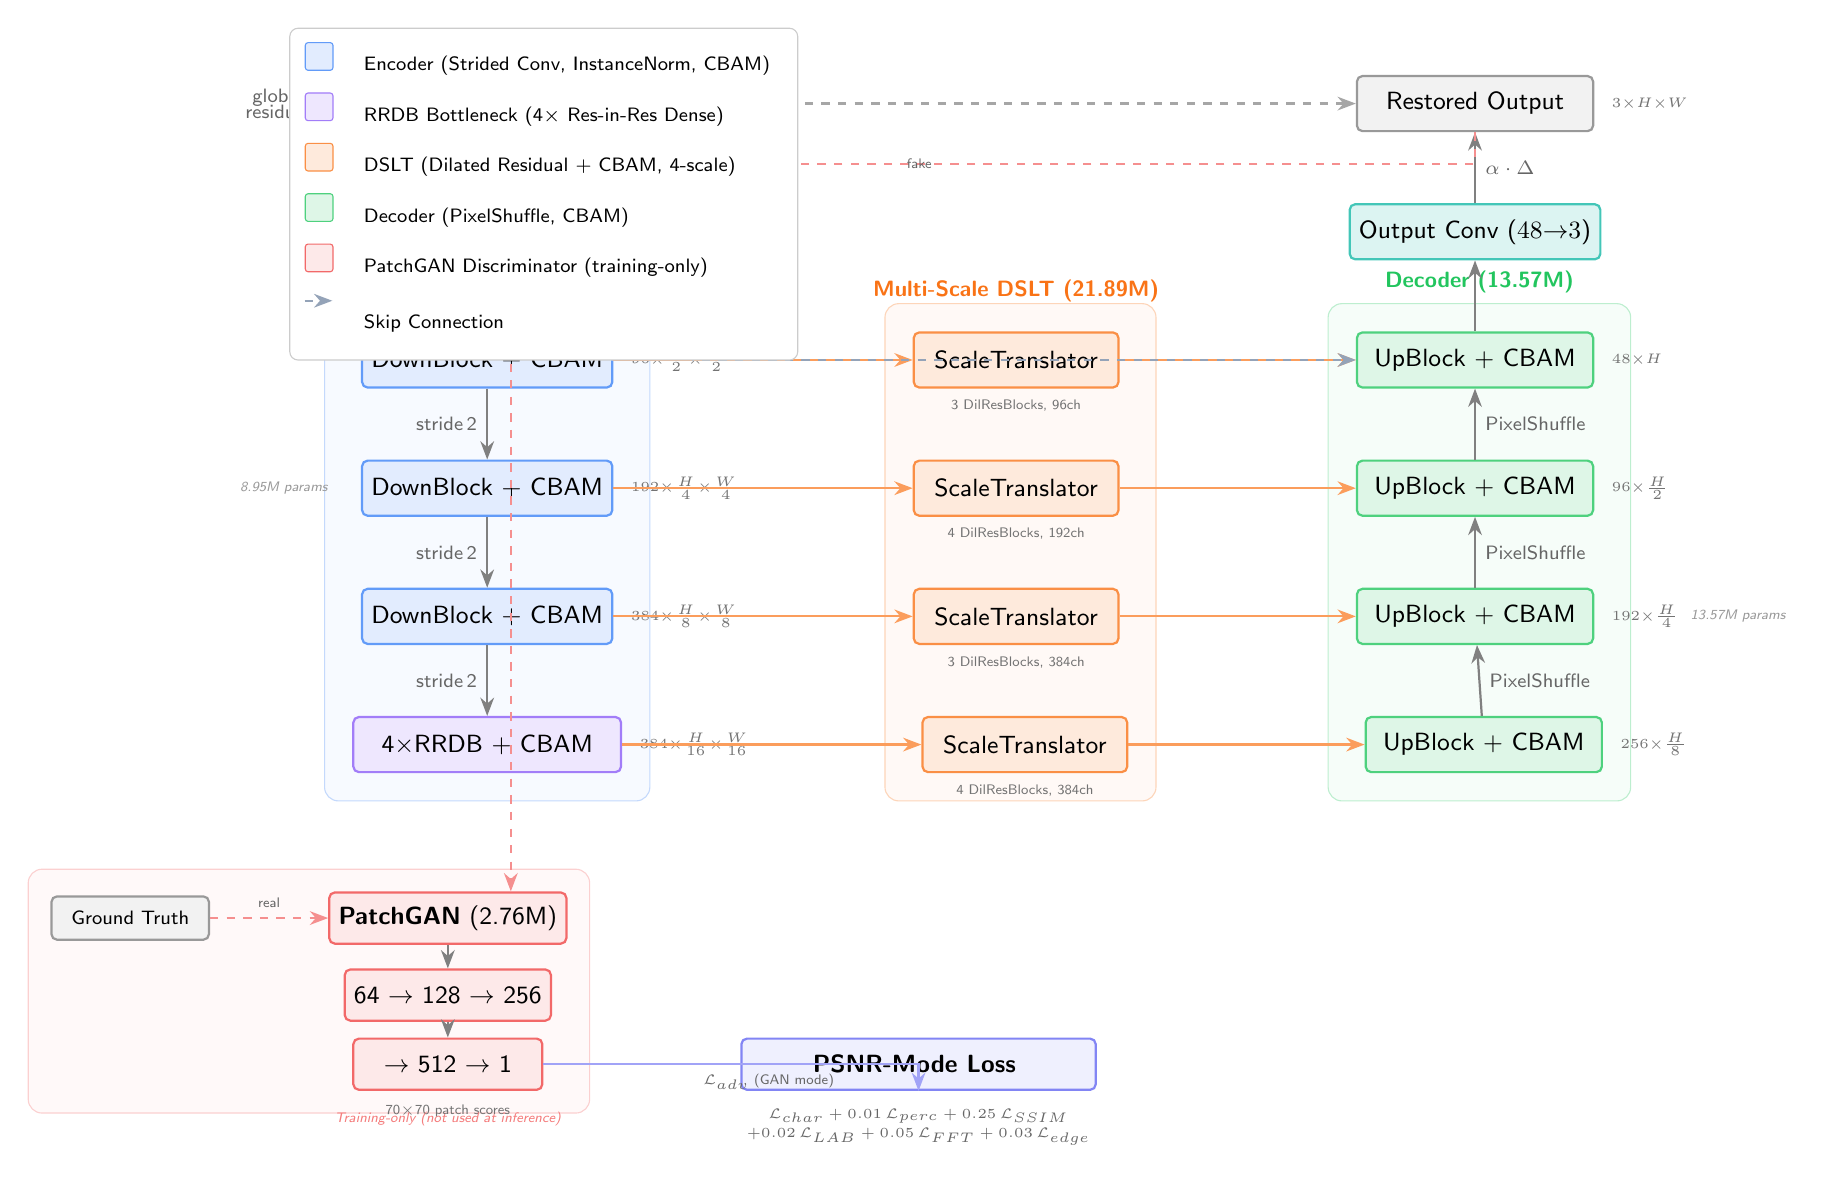
\begin{tikzpicture}[
    node distance=0.9cm and 2.0cm,
    >=Stealth,
    % ── block styles ──
    enc block/.style={
      draw=enc!80, fill=enc!15, rounded corners=2pt,
      minimum width=3.0cm, minimum height=0.7cm,
      font=\small\sffamily, align=center, thick
    },
    rrdb block/.style={
      draw=rrdb!80, fill=rrdb!15, rounded corners=2pt,
      minimum width=3.4cm, minimum height=0.7cm,
      font=\small\sffamily, align=center, thick
    },
    dslt block/.style={
      draw=dslt!80, fill=dslt!15, rounded corners=2pt,
      minimum width=2.6cm, minimum height=0.7cm,
      font=\small\sffamily, align=center, thick
    },
    dec block/.style={
      draw=dec!80, fill=dec!15, rounded corners=2pt,
      minimum width=3.0cm, minimum height=0.7cm,
      font=\small\sffamily, align=center, thick
    },
    io block/.style={
      draw=black!40, fill=black!5, rounded corners=2pt,
      minimum width=3.0cm, minimum height=0.7cm,
      font=\small\sffamily, align=center, thick
    },
    head block/.style={
      draw=head!80, fill=head!15, rounded corners=2pt,
      minimum width=3.0cm, minimum height=0.7cm,
      font=\small\sffamily, align=center, thick
    },
    gan block/.style={
      draw=gan!80, fill=gan!12, rounded corners=2pt,
      minimum width=2.8cm, minimum height=0.65cm,
      font=\small\sffamily, align=center, thick
    },
    loss block/.style={
      draw=loss!80, fill=loss!10, rounded corners=2pt,
      minimum width=3.0cm, minimum height=0.65cm,
      font=\small\sffamily, align=center, thick
    },
    dim/.style={font=\tiny\sffamily, text=black!55},
    param/.style={font=\tiny\sffamily\itshape, text=black!40},
    lbl/.style={font=\scriptsize\sffamily, text=black!60},
    arr/.style={->, thick, black!50},
    skiparr/.style={->, thick, dashed, skip},
    dsltarr/.style={->, thick, dslt!70},
    ganarr/.style={->, thick, dashed, gan!60},
]

% ============================
%  ENCODER (left column)
% ============================
\node[io block] (input) {Degraded Input};
\node[dim, right=0.1cm of input.east, anchor=west] {$3{\times}H{\times}W$};

\node[enc block, below=of input] (e1) {Conv Block + CBAM};
\node[dim, right=0.1cm of e1.east, anchor=west] {$48{\times}H{\times}W$};

\node[enc block, below=of e1] (e2) {DownBlock + CBAM};
\node[dim, right=0.1cm of e2.east, anchor=west] {$96{\times}\frac{H}{2}{\times}\frac{W}{2}$};

\node[enc block, below=of e2] (e3) {DownBlock + CBAM};
\node[dim, right=0.1cm of e3.east, anchor=west] {$192{\times}\frac{H}{4}{\times}\frac{W}{4}$};

\node[enc block, below=of e3] (e4) {DownBlock + CBAM};
\node[dim, right=0.1cm of e4.east, anchor=west] {$384{\times}\frac{H}{8}{\times}\frac{W}{8}$};

\node[rrdb block, below=of e4] (bn) {4${\times}$RRDB + CBAM};
\node[dim, right=0.1cm of bn.east, anchor=west] {$384{\times}\frac{H}{16}{\times}\frac{W}{16}$};

% ── encoder arrows ──
\draw[arr] (input) -- (e1);
\draw[arr] (e1) -- node[lbl, left] {stride\,2} (e2);
\draw[arr] (e2) -- node[lbl, left] {stride\,2} (e3);
\draw[arr] (e3) -- node[lbl, left] {stride\,2} (e4);
\draw[arr] (e4) -- node[lbl, left] {stride\,2} (bn);

% ── Encoder param label ──
\node[param, left=0.3cm of e3] {8.95M params};

% ============================
%  MULTI-SCALE DSLT (middle)
% ============================
\node[dslt block, right=3.8cm of e2] (d_e2) {ScaleTranslator};
\node[dim, below=0.02cm of d_e2] {\tiny 3 DilResBlocks, 96ch};

\node[dslt block, right=3.8cm of e3] (d_e3) {ScaleTranslator};
\node[dim, below=0.02cm of d_e3] {\tiny 4 DilResBlocks, 192ch};

\node[dslt block, right=3.8cm of e4] (d_e4) {ScaleTranslator};
\node[dim, below=0.02cm of d_e4] {\tiny 3 DilResBlocks, 384ch};

\node[dslt block, right=3.8cm of bn] (d_bn) {ScaleTranslator};
\node[dim, below=0.02cm of d_bn] {\tiny 4 DilResBlocks, 384ch};

% ── DSLT label ──
\node[font=\footnotesize\sffamily\bfseries, text=dslt, above=0.25cm of d_e2]
  {Multi-Scale DSLT (21.89M)};

% ── encoder → DSLT ──
\draw[dsltarr] (e2) -- (d_e2);
\draw[dsltarr] (e3) -- (d_e3);
\draw[dsltarr] (e4) -- (d_e4);
\draw[dsltarr] (bn) -- (d_bn);

% ============================
%  DECODER (right column)
% ============================
\node[dec block, right=3.0cm of d_bn] (u4) {UpBlock + CBAM};
\node[dim, right=0.1cm of u4.east, anchor=west] {$256{\times}\frac{H}{8}$};

\node[dec block, right=3.0cm of d_e4] (u3) {UpBlock + CBAM};
\node[dim, right=0.1cm of u3.east, anchor=west] {$192{\times}\frac{H}{4}$};

\node[dec block, right=3.0cm of d_e3] (u2) {UpBlock + CBAM};
\node[dim, right=0.1cm of u2.east, anchor=west] {$96{\times}\frac{H}{2}$};

\node[dec block, right=3.0cm of d_e2] (u1) {UpBlock + CBAM};
\node[dim, right=0.1cm of u1.east, anchor=west] {$48{\times}H$};

% ── decoder arrows ──
\draw[arr] (u4) -- node[lbl, right] {PixelShuffle} (u3);
\draw[arr] (u3) -- node[lbl, right] {PixelShuffle} (u2);
\draw[arr] (u2) -- node[lbl, right] {PixelShuffle} (u1);

% ── Decoder param label ──
\node[param, right=0.3cm of u3.east, anchor=west, xshift=0.8cm] {13.57M params};

% ── DSLT → Decoder (translated skips) ──
\draw[dsltarr] (d_bn) -- (u4);
\draw[dsltarr] (d_e4) -- (u3);
\draw[dsltarr] (d_e3) -- (u2);
\draw[dsltarr] (d_e2) -- (u1);

% ── e1 skip (direct, no DSLT) ──
\draw[skiparr] (e1.east) -- ++(1.0,0) |- (u1.west)
  node[lbl, pos=0.28, above] {e1 skip};

% ============================
%  OUTPUT HEAD
% ============================
\node[head block, above=of u1] (head) {Output Conv ($48{\to}3$)};
\draw[arr] (u1) -- (head);

\node[io block, above=of head] (output) {Restored Output};
\node[dim, right=0.1cm of output.east, anchor=west] {$3{\times}H{\times}W$};
\draw[arr] (head) -- node[lbl, right] {$\alpha \cdot \Delta$} (output);

% ── Global residual skip ──
\draw[skiparr, black!35]
  (input.west) -- ++(-0.6,0) |- (output.west)
  node[lbl, pos=0.5, left, align=center] {global\\[-2pt]residual};

% ============================
%  PATCHGAN DISCRIMINATOR
% ============================
\node[gan block, below=1.5cm of bn, xshift=-0.5cm] (disc_title) {\textbf{PatchGAN} (2.76M)};
\node[gan block, below=0.3cm of disc_title, minimum width=2.4cm] (disc1) {64 $\to$ 128 $\to$ 256};
\node[gan block, below=0.2cm of disc1, minimum width=2.4cm] (disc2) {$\to$ 512 $\to$ 1};
\node[dim, below=0.05cm of disc2] {\tiny 70$\times$70 patch scores};

\draw[arr] (disc_title) -- (disc1);
\draw[arr] (disc1) -- (disc2);

% ── Target (GT) and Output → Discriminator ──
\draw[ganarr] (output.south) -- ++(0,-0.4) -| ($(disc_title.north)+(0.8,0)$)
  node[lbl, pos=0.3, right] {\tiny fake};

\node[io block, left=1.5cm of disc_title, minimum width=2.0cm, minimum height=0.55cm]
  (gt) {\scriptsize Ground Truth};
\draw[ganarr] (gt) -- (disc_title)
  node[lbl, pos=0.5, above] {\tiny real};

% ── Training-only label ──
\node[font=\tiny\sffamily\itshape, text=gan!70, below=0.15cm of disc2]
  {Training-only (not used at inference)};

% ============================
%  LOSS FUNCTION
% ============================
\node[loss block, right=2.5cm of disc2, minimum width=4.5cm] (lossbox) {
  \textbf{PSNR-Mode Loss}
};
\node[font=\tiny\sffamily, below=0.1cm of lossbox, align=center, text=black!60] (lossdetail) {
  $\mathcal{L}_{\text{char}} + 0.01\,\mathcal{L}_{\text{perc}} + 0.25\,\mathcal{L}_{\text{SSIM}}$\\[1pt]
  $+ 0.02\,\mathcal{L}_{\text{LAB}} + 0.05\,\mathcal{L}_{\text{FFT}} + 0.03\,\mathcal{L}_{\text{edge}}$
};

\draw[arr, loss!60] (disc2.east) -| (lossbox.south)
  node[lbl, pos=0.3, below] {\tiny $\mathcal{L}_{adv}$ (GAN mode)};

% ============================
%  GROUP LABELS (background)
% ============================
\begin{scope}[on background layer]
  % Encoder
  \node[draw=enc!30, fill=enc!4, rounded corners=5pt,
        fit=(e1)(e4)(bn), inner sep=10pt,
        label={[font=\footnotesize\sffamily\bfseries, text=enc]above:Encoder (8.95M)}] {};
  % DSLT
  \node[draw=dslt!30, fill=dslt!4, rounded corners=5pt,
        fit=(d_e2)(d_bn), inner sep=10pt] {};
  % Decoder
  \node[draw=dec!30, fill=dec!4, rounded corners=5pt,
        fit=(u1)(u4), inner sep=10pt,
        label={[font=\footnotesize\sffamily\bfseries, text=dec]above:Decoder (13.57M)}] {};
  % Discriminator
  \node[draw=gan!25, fill=gan!3, rounded corners=5pt,
        fit=(disc_title)(disc2)(gt), inner sep=8pt] {};
\end{scope}


% ============================
%  LEGEND
% ============================
\matrix[draw=black!20, rounded corners=3pt, fill=white,
        column sep=6pt, row sep=1pt, inner sep=5pt,
        anchor=north west, font=\scriptsize\sffamily]
  at ($(input.north west)+(-1.0, 0.6)$)
{
  \node[fill=enc!15, draw=enc!80, minimum width=0.35cm, minimum height=0.25cm, rounded corners=1pt]{}; &
  \node{Encoder (Strided Conv, InstanceNorm, CBAM)}; \\
  \node[fill=rrdb!15, draw=rrdb!80, minimum width=0.35cm, minimum height=0.25cm, rounded corners=1pt]{}; &
  \node{RRDB Bottleneck (4$\times$ Res-in-Res Dense)}; \\
  \node[fill=dslt!15, draw=dslt!80, minimum width=0.35cm, minimum height=0.25cm, rounded corners=1pt]{}; &
  \node{DSLT (Dilated Residual + CBAM, 4-scale)}; \\
  \node[fill=dec!15, draw=dec!80, minimum width=0.35cm, minimum height=0.25cm, rounded corners=1pt]{}; &
  \node{Decoder (PixelShuffle, CBAM)}; \\
  \node[fill=gan!12, draw=gan!80, minimum width=0.35cm, minimum height=0.25cm, rounded corners=1pt]{}; &
  \node{PatchGAN Discriminator (training-only)}; \\
  \draw[skiparr] (0,0) -- (0.35,0); &
  \node{Skip Connection}; \\
};

\end{tikzpicture}
\end{document}
